% !TeX spellcheck = de_DE
\section{Finanzierung – Crowdfunding}
\subsection{Crowdsourcing vs. Crowdfunding}
\begin{itemize}
	\item \textbf{Grundidee «Crowd»:} Statt konkreter Einzelner wird einfach offen die Allgemeinheit (meist über das Internet) auf konkrete Unterstützung angesprochen.
	\item \textbf{Crowdsourcing:} Es wird offen nach Unterstützung in Form von Informationen und Dienstleistungen für eine konkrete Herausforderung gefragt. Beispiele: Programmierung: Open Source Software, User Generated Content: Social Media, Informationen: Brainstorming Plattformen z.B. Atizio
	\item \textbf{Crowdfunding:} Es wird nach finanzieller Unterstützung für ein konkretes Vorhaben gefragt. Im Gegenzug werden bestimmte Gegenleistungen angeboten.
\end{itemize}

\subsection{Crowdfunding}
Vier Arten von Crowdfunding (kategorisiert nach Gegenleistung):
\begin{itemize}
	\item \textbf{Crowdinvesting (Equity-based Crowdfunding):} Monetäre Gegenleistungen (Firmenanteile, Gewinnbeteiligungen)
	\item \textbf{Crowdlending:} Monetäre Gegenleistung (Zinszahlungen)
	\item \textbf{Reward-based Crowdfunding:} Nicht-monetäre Gegenleistungen (Symbolische Rewards, Produkt oder Dienstleistung selbst)
	\item \textbf{Crowddonating:} Nicht-monetäre Gegenleistungen (Spenden)
\end{itemize}

\subsubsection{Crowdinvesting}
\begin{itemize}
	\item Gegenleistung: Firmenanteile bzw. Gewinnbeteiligungen
	\item Vornehmlich für (skalierbare) Start-ups
\end{itemize}
\begin{itemize}
	\item \textbf{Vorteile:} Grosse Finanzierungssummen, kein zweckgebundenes Geld, Aufbau Kontaktnetzwerk zu möglichen Folgeinvestoren
	\item \textbf{Nachteile:} Mögliche Schwierigkeiten bei späterer Veräusserung, kein Feedback vom Markt oder Kunden, wenig Marketingcharakter
\end{itemize}
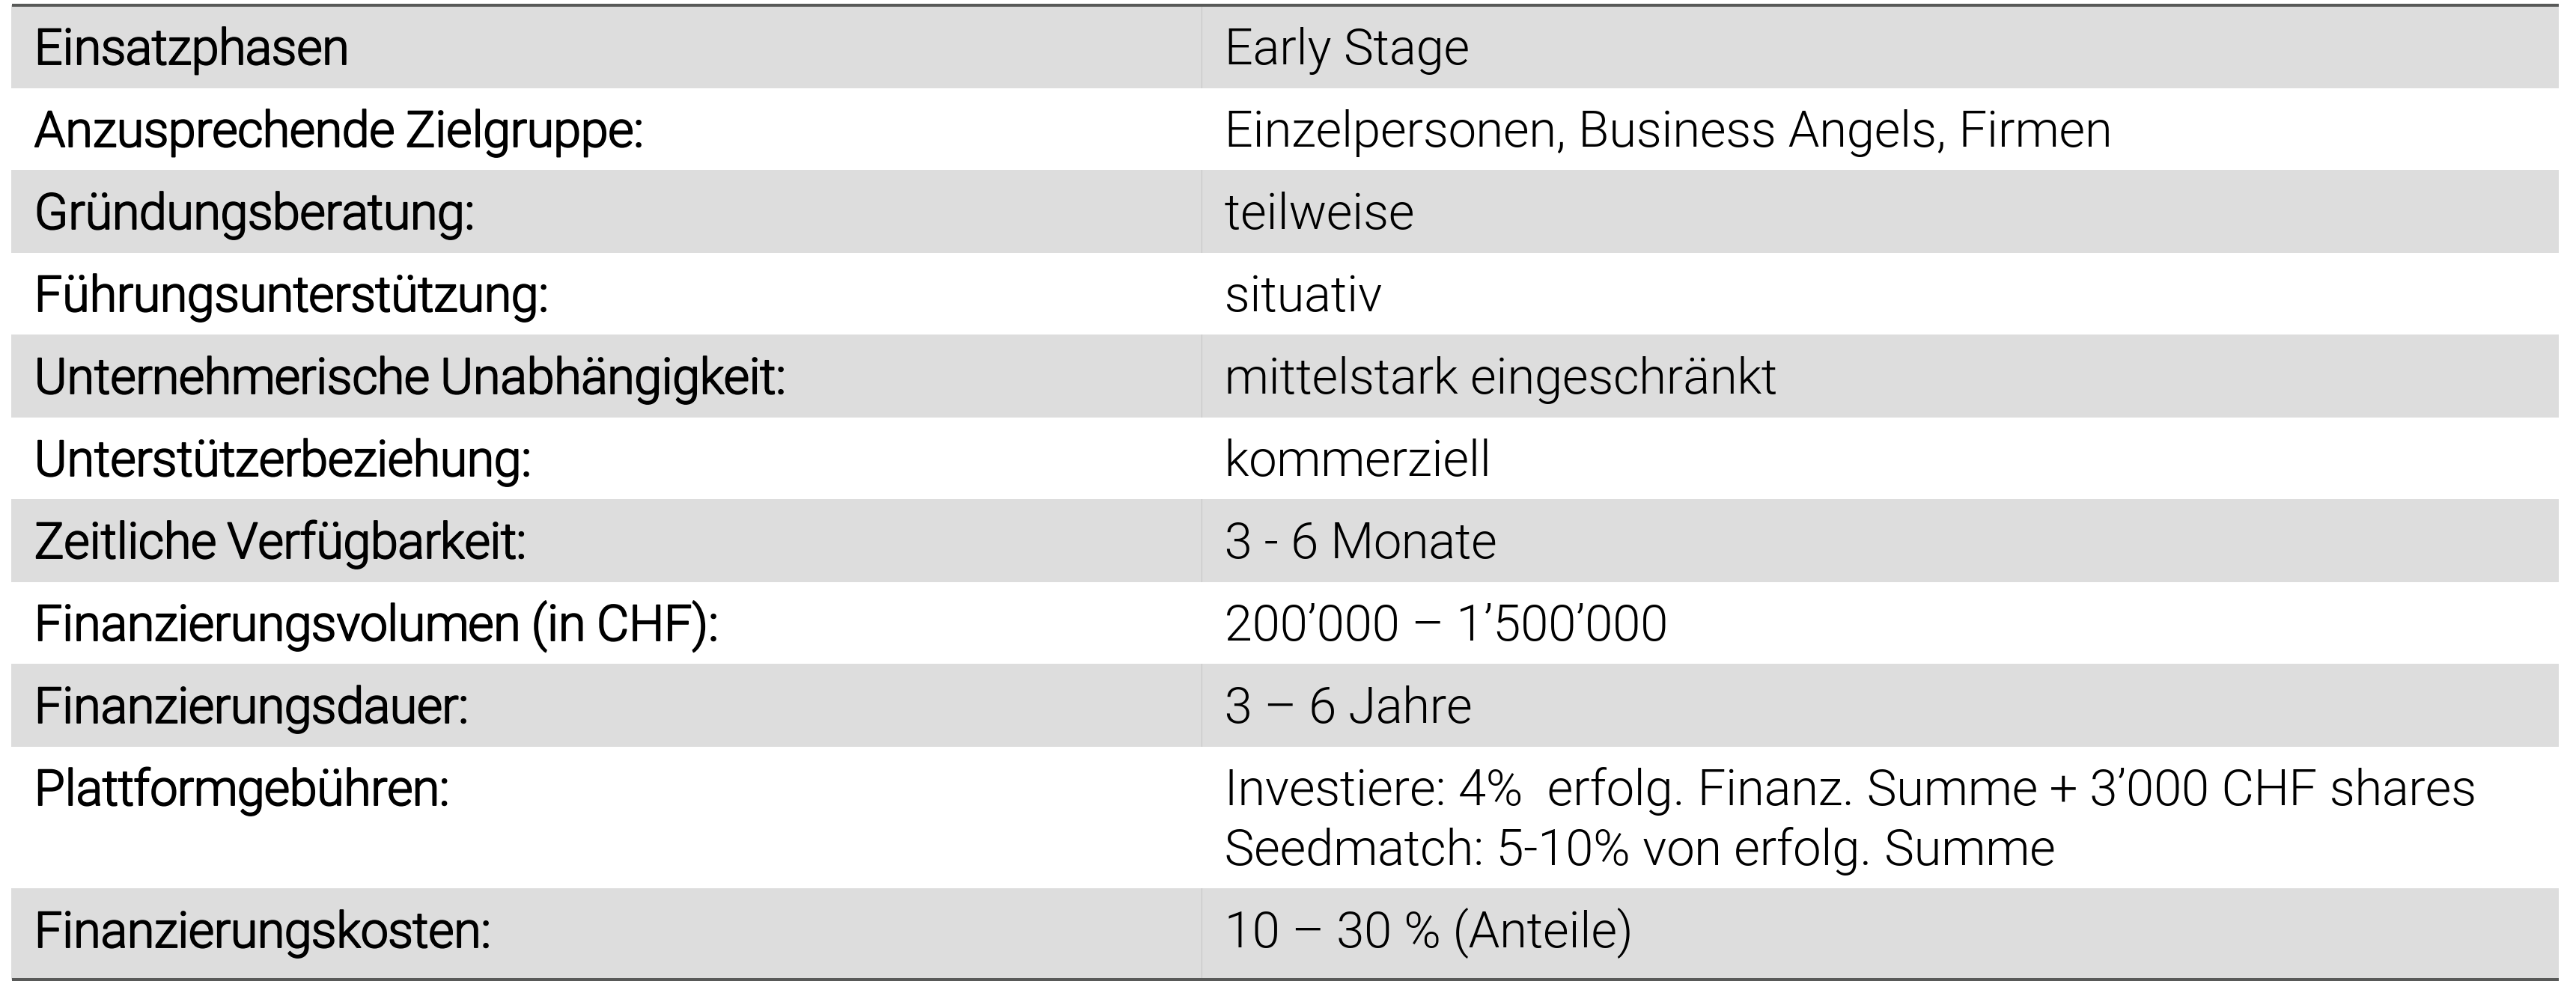
\includegraphics[width=1\linewidth]{images/crowdinvesting}

\subsubsection{Crowdlending}
Unter Crowdlending versteht man die Vergabe von Darlehen durch mehrere Personen an einen Darlehensnehmer über eine entsprechende Plattform.
\begin{itemize}
	\item Gegenleistung: bestimmte Zinsrate für ein Darlehen
	\item Risikoprüfung, kaum «Storytelling»
	\item Für Private und KMU
\end{itemize}
\begin{itemize}
	\item \textbf{Vorteile: }Geringerer Aufwand für Plattformpräsenz, schnelle Verfügbarkeit, keine Abgabe von Eigenkapitalanteilen
	\item \textbf{Nachteile:} Finanzielle Mittel sind zweckgebunden, zukünftige Kosten (Zins/Tilgung)
\end{itemize}
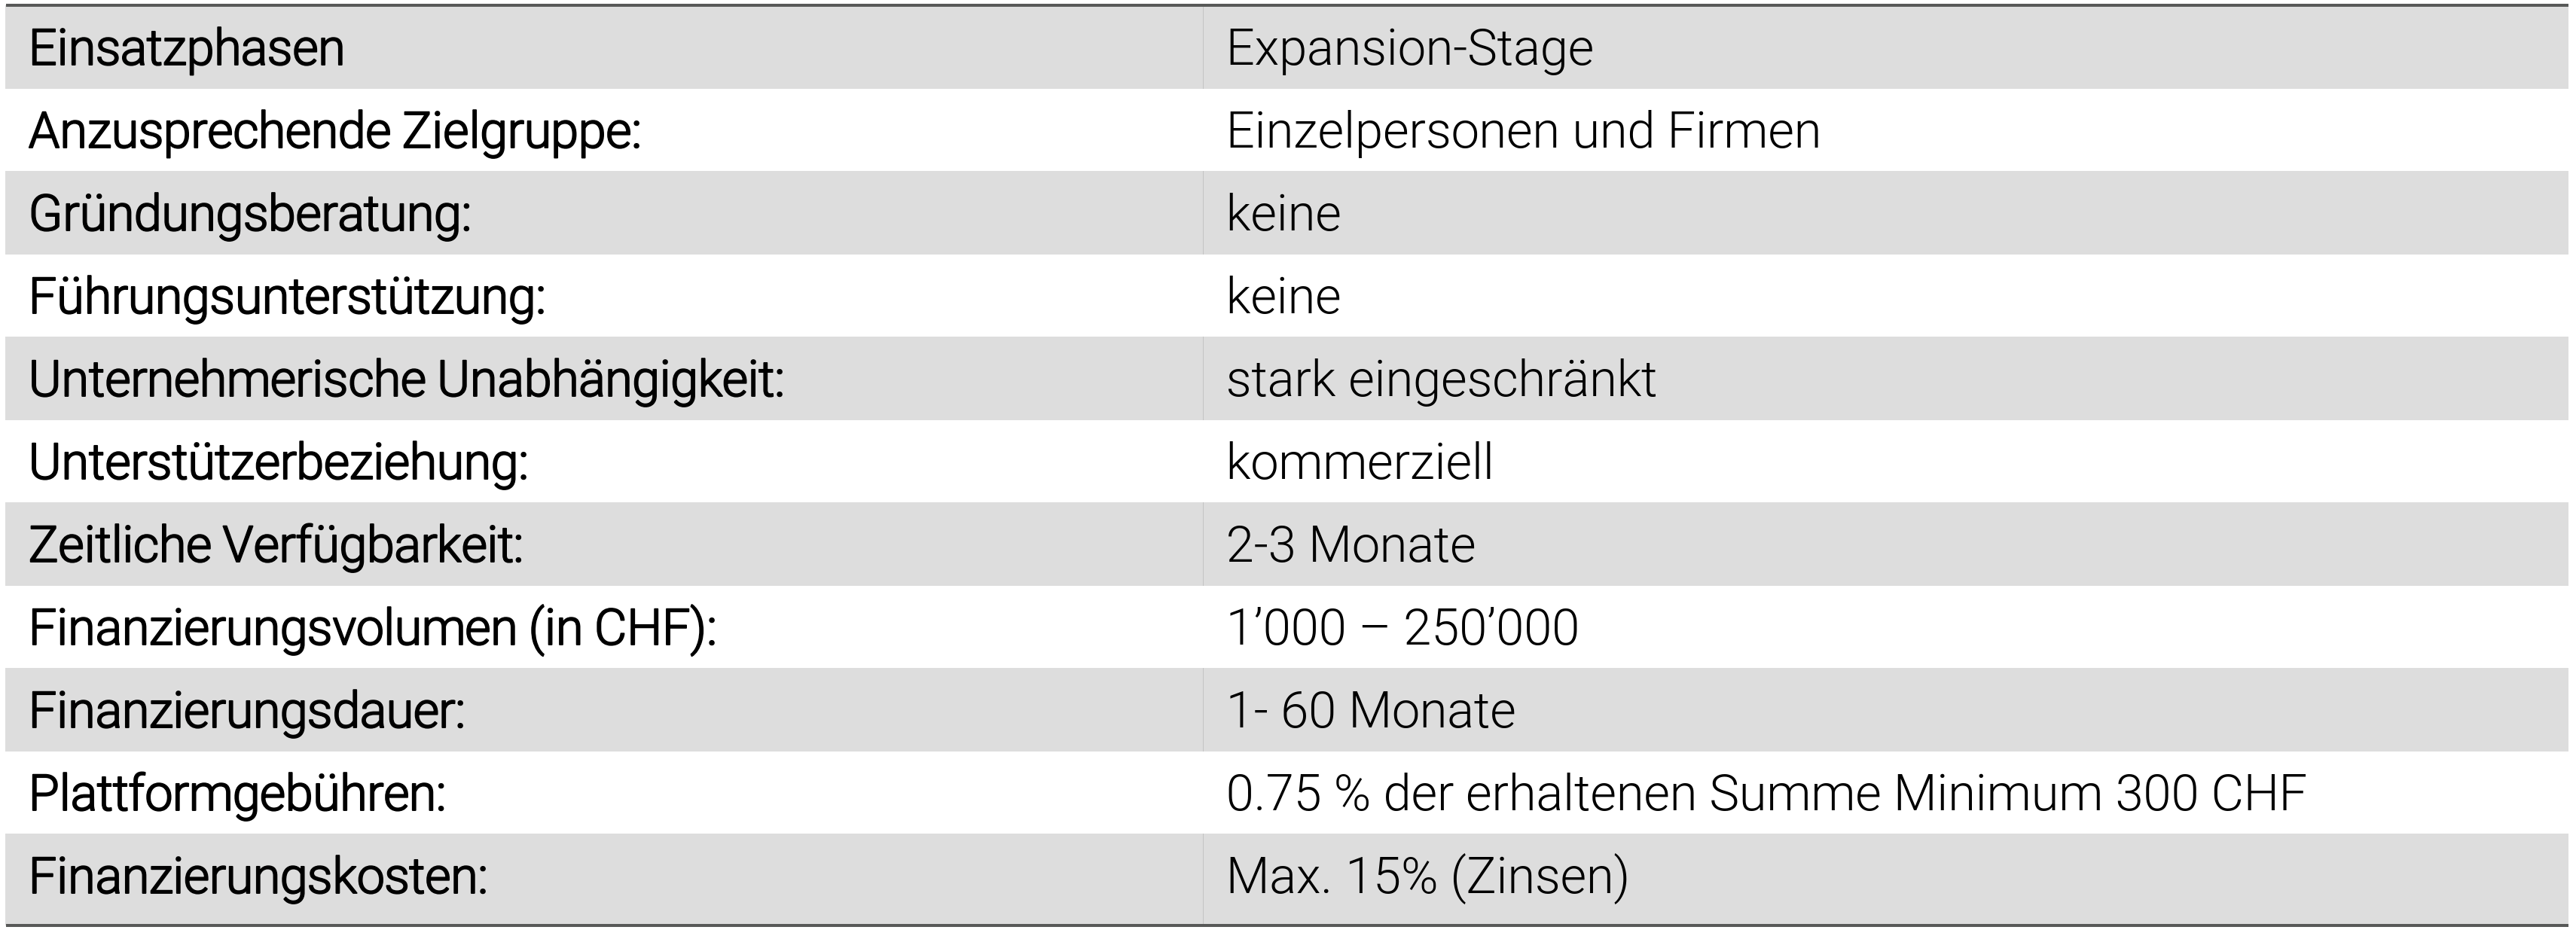
\includegraphics[width=1\linewidth]{images/crowdlending}

\subsubsection{Reward-based Crowdfunding}
\begin{itemize}
	\item Gegenleistung: Symbolische Rewards, Produkt oder Dienstleistung selbst
	\item Mehrwerte für Unternehmen: PR, Marketing, Vorabverkauf, Open Innovation, Community-Aufbau
	\item Für Private und KMU
\end{itemize}
\begin{itemize}
	\item \textbf{Vorteile:} Verschiedene Mehrwerte für Unternehmen, freie Einsatzmöglichkeit von finanziellen Mitteln, keine Abgabe von Eigenkapitalanteilen
	\item \textbf{Nachteile:} Anspruchsvolle Vorbereitung der Kampagne
\end{itemize}
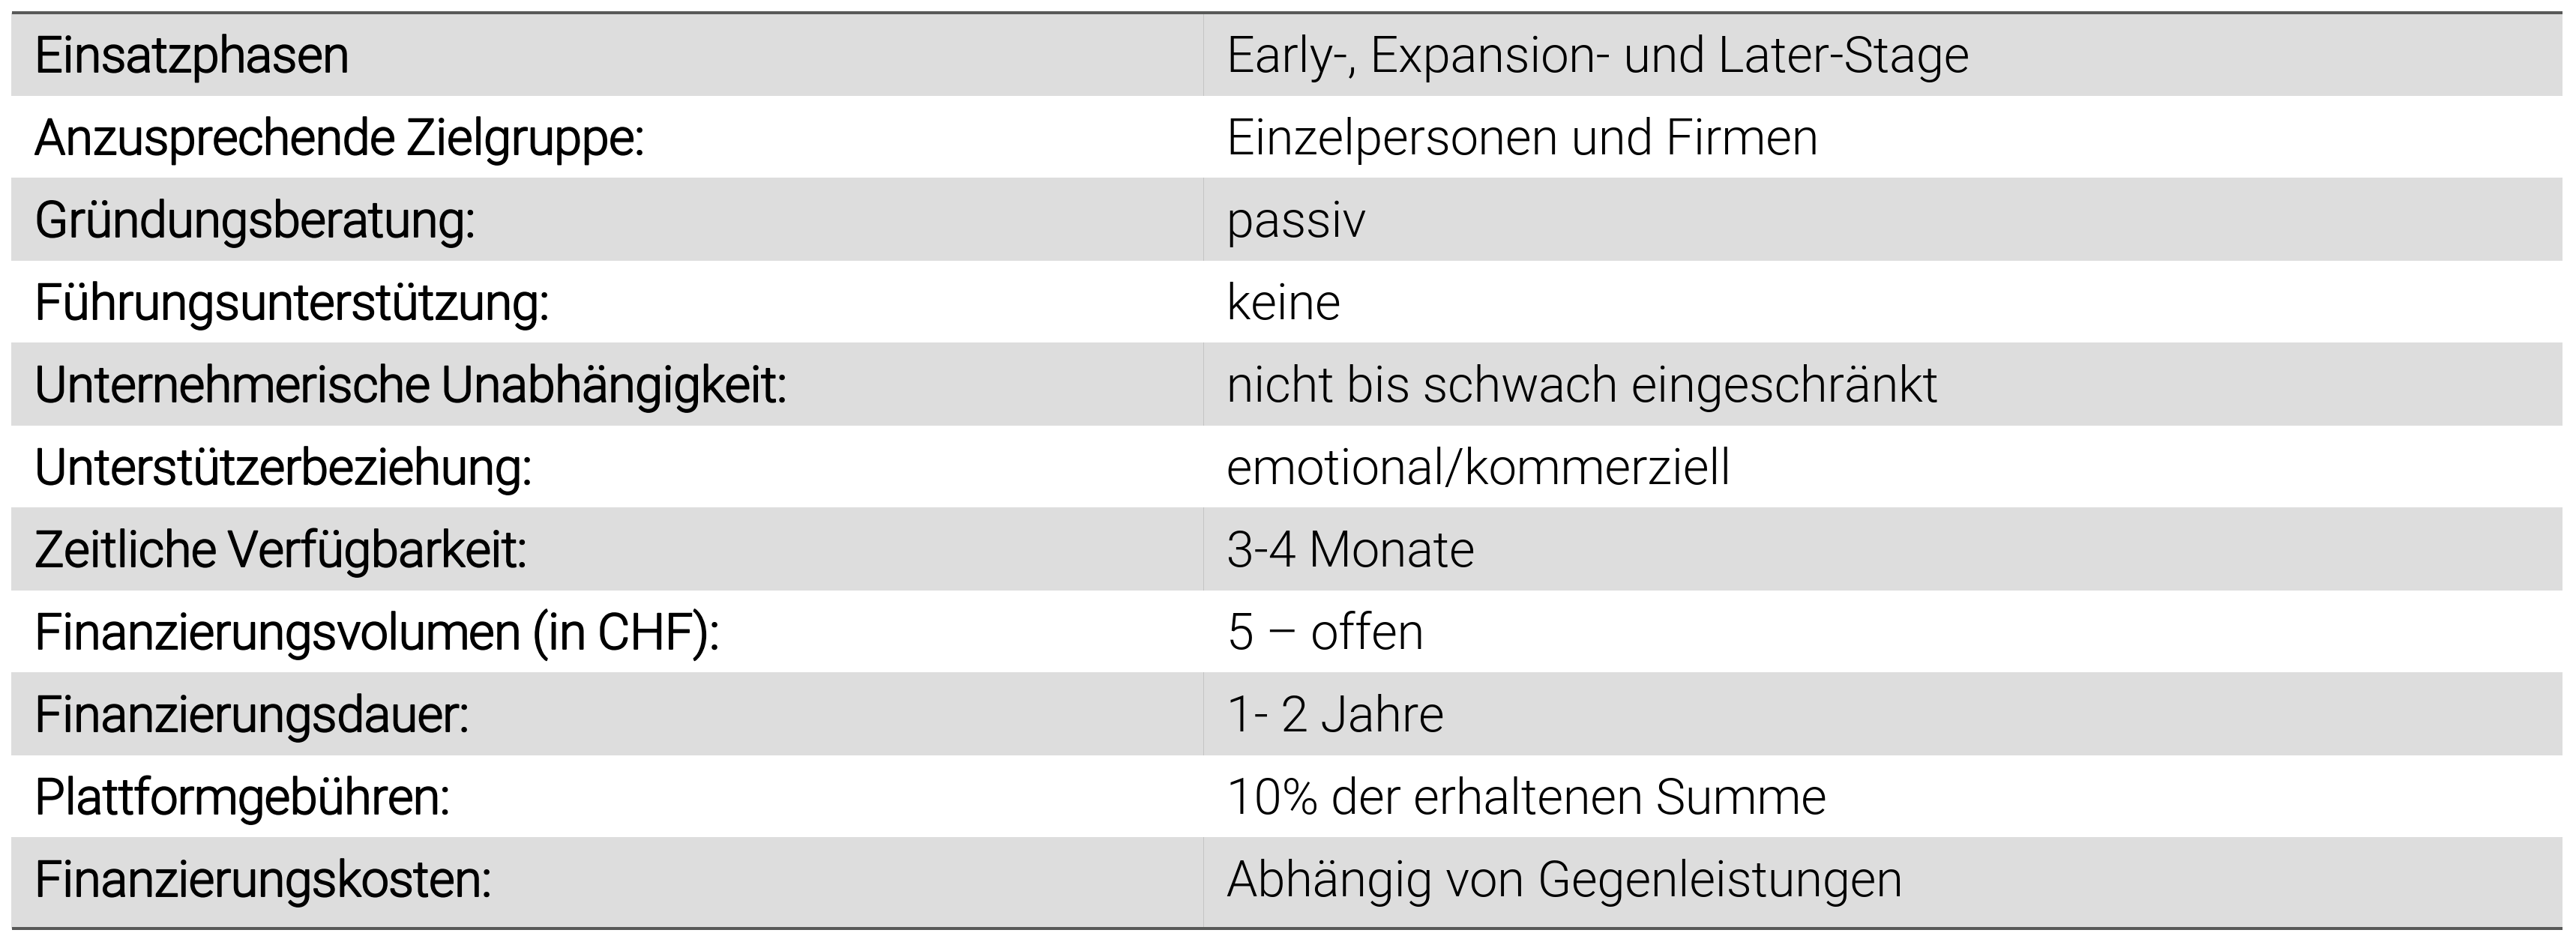
\includegraphics[width=1\linewidth]{images/crowdfunding}
